%% chapter07_slides.tex  —  Chapter 7: GeoSpatial Data
%% Nature Inspired Optimisation for Delivery Problems (2022)
%% Self-contained lecture notes formatted as Beamer slides.
%% Compile twice with: pdflatex -interaction=nonstopmode chapter07_slides.tex

\documentclass[aspectratio=169,10pt]{beamer}

\usetheme{Madrid}
\usecolortheme{seahorse}

\usepackage[utf8]{inputenc}
\usepackage[T1]{fontenc}
\usepackage{amsmath,amssymb}
\usepackage{graphicx}
\usepackage{booktabs}
\usepackage{listings}
\usepackage{xcolor}
\usepackage{microtype}
\usepackage{hyperref}
\usepackage{tikz}
\usetikzlibrary{arrows.meta,positioning,shapes.geometric}

\graphicspath{{figures/}}

%% ── listings style ──────────────────────────────────────────────
\lstset{
  language=Python,
  basicstyle=\ttfamily\scriptsize,
  numbers=left,
  numberstyle=\tiny\color{gray},
  frame=single,
  backgroundcolor=\color{gray!7},
  keywordstyle=\color{blue!70!black}\bfseries,
  commentstyle=\color{green!50!black}\itshape,
  stringstyle=\color{orange!80!black},
  breaklines=true,
  showstringspaces=false,
  tabsize=4,
}

%% ── footer ──────────────────────────────────────────────────────
\setbeamertemplate{footline}[frame number]
\setbeamertemplate{navigation symbols}{}

%% ── title slide ─────────────────────────────────────────────────
\title[Ch.7 GeoSpatial Data]{Chapter 7: GeoSpatial Data}
\subtitle{Nature Inspired Optimisation for Delivery Problems (2022)}
\author{Lecture Notes}
\date{}

% ================================================================
\begin{document}
% ================================================================

\begin{frame}
  \titlepage
\end{frame}

% ────────────────────────────────────────────────────────────────
\begin{frame}{Chapter Overview}
% ────────────────────────────────────────────────────────────────
  This chapter introduces the data types and structures that underpin
  modern digital mapping and geographic information systems (GIS).
  Understanding these foundations is essential before we can optimise
  delivery routes, because every optimisation algorithm ultimately
  relies on a faithful computer representation of the real-world road
  network.

  \vspace{0.5em}
  \begin{block}{Chapter Contents}
    \begin{enumerate}
      \item \textbf{7.1} A Brief History of Mapping
      \item \textbf{7.2} Graphics: Raster vs.\ Vector — formats, use cases
      \item \textbf{7.3} Coordinate Systems — WGS84, projections, latitude/longitude,
                          Haversine distance
      \item \textbf{7.4} Graph Theory and Networks — adjacency, weighted graphs,
                          network representation of road maps
      \item \textbf{7.5} Conclusions
    \end{enumerate}
  \end{block}

  \begin{alertblock}{Key Takeaway}
    Map data may be stored as raster images or as vector data.
    A rendering algorithm may produce raster images from vector data.
    Vector data is particularly useful because it can carry rich
    metadata --- opening hours, speed limits, turn restrictions ---
    which feed directly into graph-based routing models.
  \end{alertblock}
\end{frame}

% ================================================================
\section{7.1 A Brief History of Mapping}
% ================================================================

\begin{frame}[allowframebreaks]{7.1 A Brief History of Mapping}

  The desire to create accurate maps of our environment is one of the
  oldest human endeavours.  Archaeological evidence suggests that
  humans have been producing maps of their surroundings since
  pre-historic times, and the tradition has continued without
  interruption ever since.

  \begin{block}{Early Cartographic Milestones}
    \begin{itemize}
      \item The Babylonian \emph{Imago Mundi} tablet (c.\ 600 BCE) is one of
            the earliest surviving world maps, showing Babylon at the centre
            surrounded by a circular ocean.
      \item The Greek geographer Ptolemy (c.\ 150 CE) produced his
            \emph{Geographia}, which introduced the concept of a coordinate
            grid (latitude and longitude) to precisely locate places.
      \item Following the invention of mechanical printing in the 15th century,
            maps became commodities that could be mass-produced, traded, and
            updated — a dramatic increase in the speed of knowledge transfer.
    \end{itemize}
  \end{block}

  \framebreak

  \textbf{The Ordnance Survey and scientific cartography.}
  As surveying techniques matured, nations invested heavily in
  systematic, large-scale mapping programmes.  In the United Kingdom,
  the \emph{Ordnance Survey} (OS) was founded in 1791.  The OS still
  produces authoritative topographic maps today, and its datasets are
  widely used for navigation and infrastructure planning.

  \begin{block}{Two Core Principles from Ordnance Survey}
    \begin{itemize}
      \item \textbf{Surveying accuracy}: OS maps are measured from a fixed
            network of triangulation points, so every location has a
            precisely known coordinate.
      \item \textbf{Two-pronged offering}: OS provides both
            (a)~\emph{map data} (raw numbers describing locations and
            features) and
            (b)~\emph{mapping software} that renders those numbers into
            images humans can read.
    \end{itemize}
  \end{block}

  \framebreak

  \textbf{John Snow's 1854 cholera map.}
  One of the most celebrated early uses of spatial data analysis is
  physician John Snow's investigation of a cholera outbreak in the
  Soho district of London.  By plotting the home addresses of cholera
  victims on a street map, Snow discovered that cases clustered
  tightly around a single water pump on Broad Street.  His insight
  --- that the \emph{spatial pattern} of a disease reveals its
  cause --- was revolutionary.  He argued that cholera was a
  water-borne illness at a time when the prevailing medical view held
  that it spread through ``bad air'' (miasma).

  \begin{exampleblock}{Worked Example: Snow's Spatial Reasoning}
    \begin{itemize}
      \item Snow drew a map with each cholera death marked as a small bar
            stacked at the victim's address.
      \item He then drew concentric circles around the Broad Street pump.
      \item The vast majority of deaths fell within a short walking distance
            of that pump.
      \item Removal of the pump handle ended the outbreak --- a classic
            demonstration that a map, combined with careful reasoning, can
            drive a life-saving decision.
    \end{itemize}
  \end{exampleblock}

  \framebreak

  \textbf{Booth's Poverty Maps (1889).}
  Charles Booth produced a series of maps of London in which every
  street was colour-coded according to the socio-economic status of
  its inhabitants.  This project --- arguably the first large-scale
  social survey in history --- showed that geospatial data could
  illuminate inequalities, not just physical terrain.

  \begin{center}
    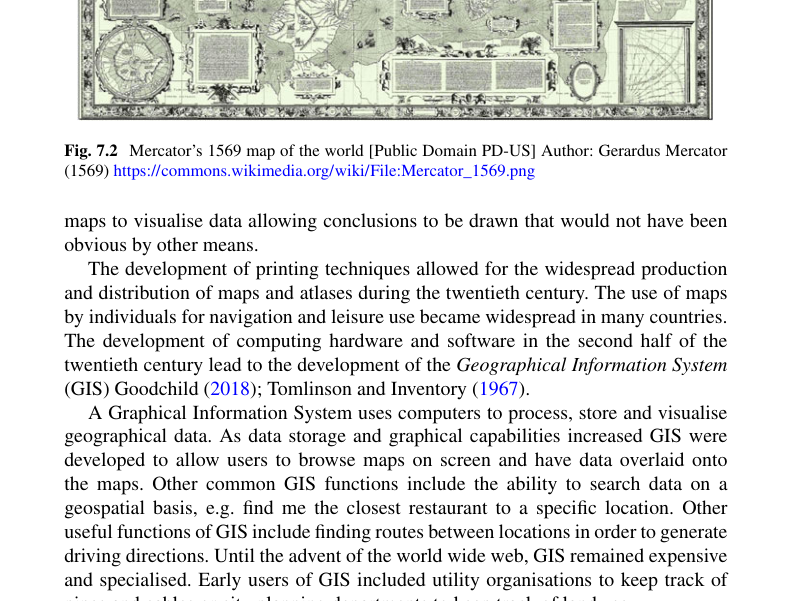
\includegraphics[width=0.62\textwidth]{fig_booth_map_crop.png}
  \end{center}
  \vspace{-0.3em}
  {\footnotesize \textit{An extract from Booth's 1889 Descriptive Map of London Poverty.
  Different colours represent different wealth categories, from black
  (lowest class, vicious, semi-criminal) through yellow (upper-middle
  and upper class).  This is a forerunner of modern choropleth mapping.}}

  \framebreak

  \textbf{The rise of digital web mapping.}
  The development of printing technology in the 15th century made maps
  widely available for the first time; the internet produced a second
  revolution of comparable magnitude.  Today, map-based web services
  allow anyone to query, display, and interact with geospatial data in
  a browser or mobile app.

  \begin{block}{Key Developments in Digital Mapping}
    \begin{itemize}
      \item \textbf{Commercial web maps} (Google Maps, Apple Maps, Bing Maps):
            satellite imagery, real-time traffic, street-level photography,
            turn-by-turn navigation.
      \item \textbf{OpenStreetMap (OSM)}: a collaborative, volunteer-created
            map of the entire world, freely available under an open licence.
            OSM allows any user to add or correct map data, and its datasets
            underpin a huge range of applications, including many
            open-source routing engines used in delivery optimisation.
      \item \textbf{GPS and mobile devices}: the widespread availability of
            GPS receivers in smartphones has transformed users into data
            contributors, feeding real-time location data back into
            mapping platforms.
    \end{itemize}
  \end{block}

  \begin{alertblock}{Key Insight}
    Modern geospatial data pipelines for delivery optimisation typically
    start with an open dataset such as OSM and transform it into a
    graph structure suitable for a routing algorithm.  Understanding
    where this data comes from --- and its potential inaccuracies ---
    is important when designing robust systems.
  \end{alertblock}

\end{frame}

% ================================================================
\section{7.2 Graphics: Raster vs.\ Vector}
% ================================================================

\begin{frame}[allowframebreaks]{7.2 Raster Graphics}

  Before we can talk about storing or manipulating map data, we need
  to understand the two fundamental ways in which \emph{any} graphical
  information can be represented in a computer: as a
  \textbf{raster image} or as \textbf{vector data}.

  \begin{block}{Definition: Raster Image}
    A raster image is a rectangular grid of individual picture elements
    called \textbf{pixels} (short for ``picture elements'').  Each pixel
    stores a colour value --- for example, as three numbers representing
    the intensities of Red, Green, and Blue light (an RGB triplet).
    The full image is nothing more than a very large 2D array of such
    numbers.
  \end{block}

  \framebreak

  \textbf{Resolution and the zoom problem.}
  The visual quality of a raster image is determined by its
  \textbf{resolution} --- the number of pixels per unit area.
  A high-resolution image has more pixels and therefore more spatial
  detail.  However, raster images suffer from a fundamental
  limitation: if you zoom in beyond the native resolution, the
  individual pixels become visible as blocky squares, and the image
  looks degraded.  This is because the image literally contains no
  more information at finer scales; the data has been discarded at
  capture time.

  \begin{block}{Common Raster File Formats}
    \begin{itemize}
      \item \textbf{PNG} (Portable Network Graphics): lossless
            compression, supports transparency, excellent for maps with
            sharp edges and text.
      \item \textbf{JPEG} (Joint Photographic Experts Group): lossy
            compression, small file sizes, best for photographs but
            introduces artefacts at sharp boundaries.
      \item \textbf{TIFF} (Tagged Image File Format): lossless, supports
            metadata and multiple layers; widely used in professional GIS.
      \item \textbf{GeoTIFF}: a TIFF that embeds geographic coordinate
            information, so each pixel can be mapped to a real-world
            location.
    \end{itemize}
  \end{block}

  \framebreak

  \textbf{Map tiles.}
  Web mapping services such as Google Maps and OpenStreetMap serve
  their raster data as a pyramid of pre-rendered image tiles.  At
  each zoom level, the world is divided into a grid of square tiles
  (typically 256$\times$256 pixels each).  When you pan or zoom in
  the browser, the client downloads only the tiles that are currently
  visible.  This tile-pyramid approach makes it feasible to deliver
  planetary-scale raster data to billions of users on demand.

\end{frame}

% ────────────────────────────────────────────────────────────────
\begin{frame}[allowframebreaks]{7.2 Vector Graphics}
% ────────────────────────────────────────────────────────────────

  Rather than storing a dense grid of pixel colours, a
  \textbf{vector} representation stores the \emph{mathematical
  description} of geometric shapes: points, lines, curves, and
  polygons, each defined by a set of coordinates.

  \begin{block}{Definition: Vector Graphics}
    In a vector image, every feature is described by
    \begin{itemize}
      \item the \textbf{type} of shape (point, line, polygon, arc),
      \item the \textbf{coordinates} of its control points or vertices,
      \item optional \textbf{attributes} such as stroke colour, fill
            colour, and line width.
    \end{itemize}
    When the image is displayed, a \emph{rendering engine} converts
    these geometric descriptions into the pixel grid that the screen
    can show.
  \end{block}

  \textbf{Infinite zoom, finite metadata.}
  Because a vector representation stores the geometry analytically,
  zooming in does not degrade quality --- the rendering engine
  simply re-computes the rasterised output at the new scale.
  More importantly for GIS applications, each feature in a vector
  file can carry arbitrary \textbf{metadata}: a road segment might
  store its name, road classification (motorway, A-road, footpath),
  speed limit, and the opening times of shops along it.

  \begin{center}
    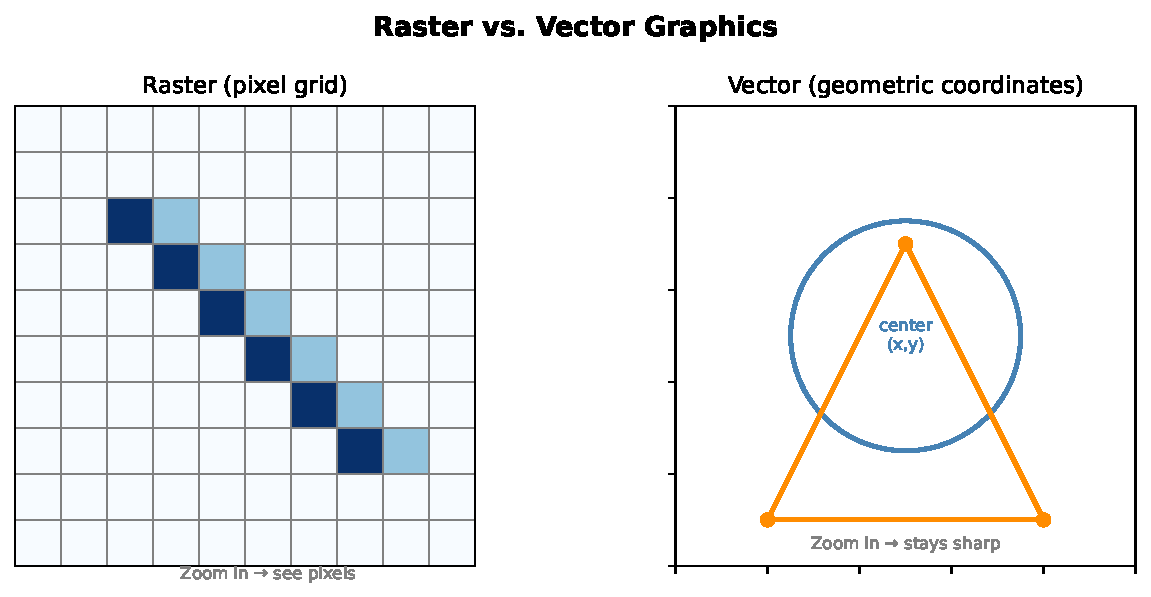
\includegraphics[width=0.75\textwidth]{raster_vs_vector.pdf}
  \end{center}
  {\footnotesize Left: A raster image zoomed in reveals individual pixels.
   Right: A vector image is defined by coordinates and remains sharp
   at any zoom level.}

  \framebreak

  \begin{block}{Common Vector File Formats}
    \begin{itemize}
      \item \textbf{SVG} (Scalable Vector Graphics): an XML-based format
            designed for the web.  A circle is literally written as
            \texttt{<circle cx="100" cy="100" r="50"/>}.  Because it is
            plain text, SVG files are easy to create, edit, and embed in
            web pages.
      \item \textbf{GeoJSON}: a JSON-based standard for encoding geographic
            features (points, lines, polygons) together with their
            non-spatial attributes.  Widely used in web GIS and APIs.
      \item \textbf{Shapefile}: the longstanding industry standard from
            Esri, used in desktop GIS software such as ArcGIS.
            A Shapefile is actually a collection of at least three
            files (\texttt{.shp}, \texttt{.dbf}, \texttt{.shx}) stored
            together.
      \item \textbf{OSM (OpenStreetMap) XML}: an open format that encodes
            the full OSM data model --- nodes, ways, and relations ---
            in XML.  This is the format used when you download an area
            from OpenStreetMap for offline use.
    \end{itemize}
  \end{block}

  \begin{center}
    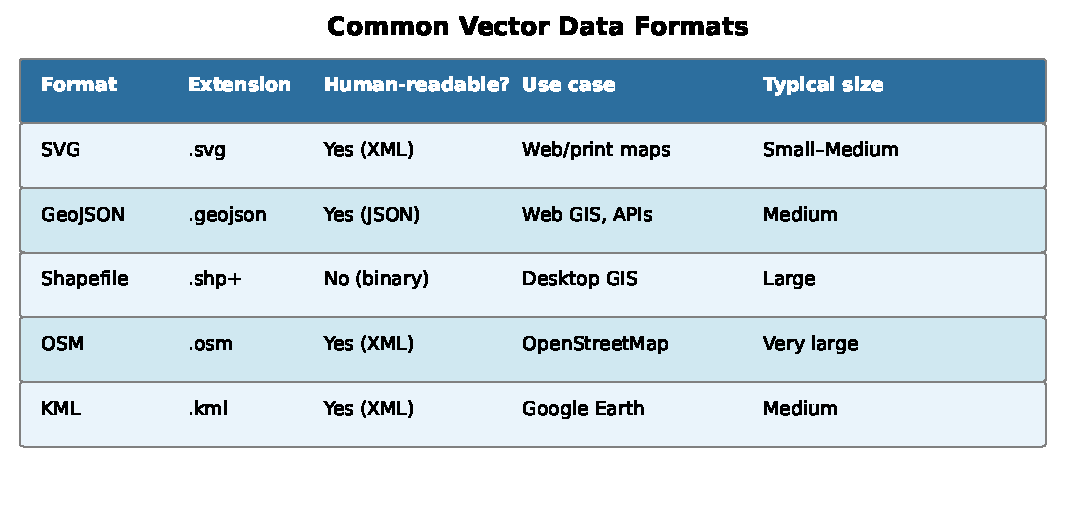
\includegraphics[width=0.80\textwidth]{vector_formats.pdf}
  \end{center}

  \framebreak

  \textbf{GeoJSON: a concrete example.}
  The following snippet shows how a road segment might be encoded as
  a GeoJSON \texttt{LineString} feature.  Notice how geometry
  (the coordinate pairs) and metadata (road name, speed limit) live
  side-by-side in the same document.

\end{frame}

% ────────────────────────────────────────────────────────────────
\begin{frame}[fragile]{Python: Reading a GeoJSON Vector File}
% ────────────────────────────────────────────────────────────────

\begin{lstlisting}[caption={GeoJSON structure and reading it with Python}]
import json

# A minimal GeoJSON file representing a road segment
geojson_text = """
{
  "type": "FeatureCollection",
  "features": [
    {
      "type": "Feature",
      "geometry": {
        "type": "LineString",
        "coordinates": [
          [-3.19, 55.95],
          [-2.90, 55.87],
          [-0.13, 51.51]
        ]
      },
      "properties": {
        "name": "A1 Road",
        "maxspeed": 70,
        "highway": "trunk"
      }
    }
  ]
}
"""

data = json.loads(geojson_text)

# Access the first feature
feature = data['features'][0]
coords   = feature['geometry']['coordinates']   # list of [lon, lat] pairs
name     = feature['properties']['name']        # "A1 Road"
speed    = feature['properties']['maxspeed']    # 70 (mph)

print(f"Road: {name}")
print(f"Speed limit: {speed} mph")
print(f"Number of coordinate points: {len(coords)}")
# Output:
# Road: A1 Road
# Speed limit: 70 mph
# Number of coordinate points: 3
\end{lstlisting}

  Notice that coordinates are stored as \texttt{[longitude, latitude]}
  pairs (note the order: longitude first, latitude second --- a common
  source of confusion).  The \texttt{properties} dictionary can hold
  any attributes relevant to the feature.

\end{frame}

% ────────────────────────────────────────────────────────────────
\begin{frame}[fragile]{Python: Reading OSM Data with OSMnx}
% ────────────────────────────────────────────────────────────────

  OpenStreetMap data can be downloaded and converted into a Python
  graph structure using the \texttt{osmnx} library.  The library
  handles all the complexities of the OSM data model and returns a
  \texttt{networkx} graph object that is immediately usable for
  routing.

\begin{lstlisting}[caption={Downloading and inspecting an OSM road network}]
import osmnx as ox

# Download the road network for a named place
# 'drive' means only driveable streets are included
G = ox.graph_from_place('Edinburgh, UK', network_type='drive')

# Basic statistics
print(f"Nodes (junctions): {len(G.nodes)}")
print(f"Edges (road segments): {len(G.edges)}")

# Each edge has attributes loaded from the OSM vector data
# For example, inspect the first edge:
u, v, data = list(G.edges(data=True))[0]
print(f"Edge {u} -> {v}")
print(f"  Street name : {data.get('name', 'unnamed')}")
print(f"  Length (m)  : {data.get('length', '?')}")
print(f"  Max speed   : {data.get('maxspeed', 'not set')}")
print(f"  Highway type: {data.get('highway', '?')}")

# Save the graph as a shapefile (vector format) for use in GIS tools
ox.save_graph_shapefile(G, filepath='edinburgh_graph')
\end{lstlisting}

  The output will report thousands of nodes (road junctions) and
  tens of thousands of edges (road segments), illustrating why
  scalable data structures (Section 7.4) are essential.

\end{frame}

% ================================================================
\section{7.3 Coordinate Systems}
% ================================================================

\begin{frame}[allowframebreaks]{7.3 Coordinate Systems: WGS84}

  A \textbf{coordinate system} is a mathematical framework that assigns
  a unique pair (or triple) of numbers to every point on Earth.
  Without a well-defined coordinate system, two people trying to
  specify the same location might use incompatible numbers.

  \begin{block}{Definition: WGS84 (World Geodetic System 1984)}
    WGS84 is the global coordinate standard used by GPS (Global
    Positioning System) and by most modern mapping applications.
    It models the Earth as an oblate spheroid --- a sphere that is
    very slightly flattened at the poles --- and defines
    \begin{itemize}
      \item \textbf{Latitude} $\phi$ (phi): the angle north or south of
            the equator (the imaginary line midway between the poles).
            Ranges from $-90^{\circ}$ (South Pole) to $+90^{\circ}$ (North Pole).
            The equator is $\phi = 0^{\circ}$.
      \item \textbf{Longitude} $\lambda$ (lambda): the angle east or
            west of the \emph{prime meridian}, an arbitrary reference
            line passing through Greenwich, London.
            Ranges from $-180^{\circ}$ to $+180^{\circ}$.
      \item \textbf{Altitude} $h$: the height above the WGS84 reference
            ellipsoid, in metres.
    \end{itemize}
  \end{block}

  \begin{center}
    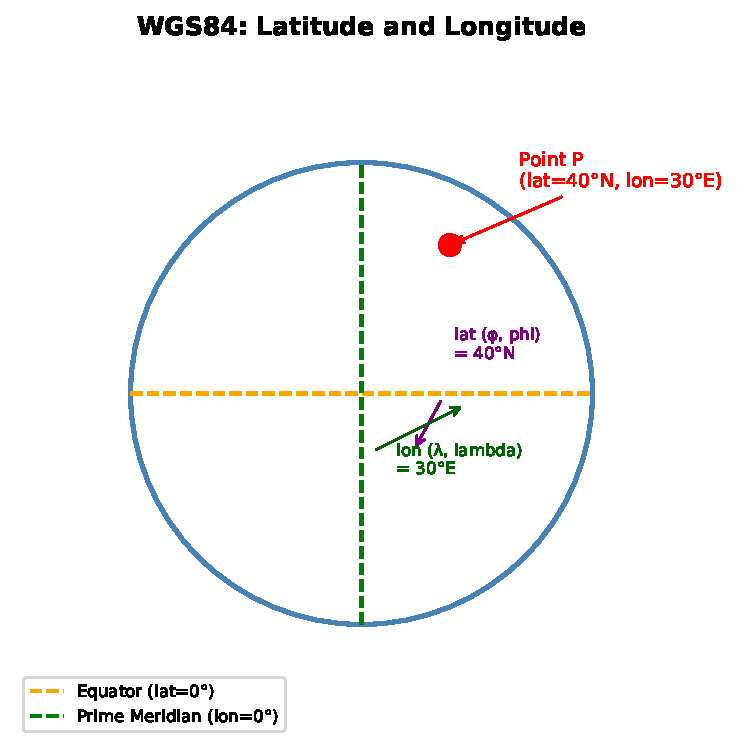
\includegraphics[width=0.55\textwidth]{coordinate_system.pdf}
  \end{center}

  \framebreak

  \textbf{How to read a coordinate pair.}
  A latitude/longitude pair such as $(55.95^{\circ}\text{N},\ 3.19^{\circ}\text{W})$
  tells us:
  \begin{itemize}
    \item $55.95^{\circ}$ north of the equator (closer to the North Pole than
          to the equator, since the equator is $0^{\circ}$ and the pole is
          $90^{\circ}$).
    \item $3.19^{\circ}$ west of the Greenwich meridian (a very small angle
          --- this is roughly the width of Scotland east-to-west near
          Edinburgh).
  \end{itemize}

  \begin{exampleblock}{Worked Example: Notable Coordinates}
    \begin{tabular}{lrr}
      \toprule
      City & Latitude $\phi$ & Longitude $\lambda$ \\
      \midrule
      Edinburgh, UK   & $55.95^{\circ}$\,N & $3.19^{\circ}$\,W \\
      London, UK      & $51.51^{\circ}$\,N & $0.13^{\circ}$\,W \\
      Paris, France   & $48.86^{\circ}$\,N & $2.35^{\circ}$\,E \\
      New York, USA   & $40.71^{\circ}$\,N & $74.01^{\circ}$\,W \\
      Sydney, Australia & $33.87^{\circ}$\,S & $151.21^{\circ}$\,E \\
      \bottomrule
    \end{tabular}

    \vspace{0.4em}
    Notice that Edinburgh lies about $4.5^{\circ}$ of latitude north of
    London --- roughly the same angular distance as driving about
    500\,km northward.
  \end{exampleblock}

  \framebreak

  \textbf{Projections: from sphere to flat map.}
  A flat map is a \emph{projection} of the curved Earth's surface
  onto a plane.  Every projection introduces some distortion ---
  it is mathematically impossible to flatten a sphere without
  stretching or compressing some regions.  Different projections
  preserve different properties:

  \begin{block}{Common Map Projections}
    \begin{itemize}
      \item \textbf{Mercator}: preserves angles (shapes of small
            regions are correct) but greatly exaggerates the size of
            land near the poles.  Greenland appears as large as Africa
            on a Mercator map, even though Africa is about 14 times
            larger.  Widely used for navigation because a straight line
            on the map corresponds to a constant compass bearing.
      \item \textbf{Equal-area projections} (e.g.\ Mollweide,
            Albers): preserve the relative sizes of regions at the
            cost of distorting shapes.  Useful for thematic maps
            showing, e.g., population density.
      \item \textbf{Transverse Mercator / UTM}: the UK's Ordnance
            Survey uses a Transverse Mercator projection that gives
            accurate distances and areas for a specific band of
            longitude.
    \end{itemize}
  \end{block}

  \textbf{For delivery optimisation}, latitude and longitude are
  usually sufficient for specifying locations, and the Haversine
  formula (Section~7.3) gives accurate straight-line (``as the crow
  flies'') distances between pairs of coordinate points anywhere on
  the globe.

  \framebreak

  \textbf{GPS and mobile positioning.}
  The latitude/longitude system allows mobile devices to become
  location-aware.  GPS receivers measure signals from a constellation
  of satellites to triangulate their position on the Earth's surface.
  This capability, combined with web mapping services, has enabled
  \begin{itemize}
    \item turn-by-turn navigation apps;
    \item real-time fleet tracking for delivery vehicles;
    \item crowd-sourced map improvement (e.g.\ OSM contributors who
          record their GPS tracks while walking or cycling).
  \end{itemize}

\end{frame}

% ────────────────────────────────────────────────────────────────
\begin{frame}[allowframebreaks]{7.3 Haversine Distance Formula}
% ────────────────────────────────────────────────────────────────

  When we know the latitude and longitude of two points on the Earth's
  surface, we want to compute the straight-line \emph{great-circle
  distance} between them --- the shortest path along the Earth's
  curved surface, as opposed to a path through the interior of the
  planet.

  \textbf{Why not just use Pythagoras?}
  If the two points are very close together (a few kilometres), using
  the Euclidean (flat-earth) formula gives a reasonable approximation.
  But for longer distances, the curvature of the Earth introduces
  significant errors.  The Haversine formula accounts for this
  curvature exactly.

  \begin{block}{The Haversine Formula}
    Given two points with coordinates
    $(\phi_1, \lambda_1)$ and $(\phi_2, \lambda_2)$
    (all angles in \emph{radians}), define:
    \[
      a = \sin^2\!\!\left(\frac{\Delta\phi}{2}\right)
          + \cos(\phi_1)\,\cos(\phi_2)\,\sin^2\!\!\left(\frac{\Delta\lambda}{2}\right)
    \]
    where
    $\Delta\phi = \phi_2 - \phi_1$ (delta-phi, the difference in latitude)
    and
    $\Delta\lambda = \lambda_2 - \lambda_1$ (delta-lambda, the difference
    in longitude).  Then:
    \[
      c = 2\,\mathrm{atan2}\!\left(\sqrt{a},\, \sqrt{1-a}\right)
    \]
    \[
      d = R \times c
    \]
    where $R \approx 6{,}371$\,km is the mean radius of the Earth,
    $c$ (the central angle, in radians) is the angular separation
    of the two points as seen from the Earth's centre,
    and $d$ is the great-circle distance in kilometres.
  \end{block}

  \framebreak

  \begin{block}{Notation Guide}
    \begin{itemize}
      \item $\phi$ (phi): latitude in radians.  To convert from
            degrees: $\phi = \text{degrees} \times \pi / 180$.
      \item $\lambda$ (lambda): longitude in radians.
      \item $\Delta\phi$ (delta-phi): the difference in latitude
            between the two points, in radians.
      \item $\Delta\lambda$ (delta-lambda): the difference in longitude,
            in radians.
      \item $\sin$ (sine): a trigonometric function.
            $\sin(\theta)$ (theta) ranges between $-1$ and $+1$.
      \item $\cos$ (cosine): another trigonometric function.
            $\cos(\theta)$ also ranges between $-1$ and $+1$.
      \item $\mathrm{atan2}(y, x)$: the ``two-argument arctangent'',
            which gives the angle whose tangent is $y/x$, taking
            the correct quadrant into account.
      \item $R$: the mean radius of the Earth, approximately
            $6{,}371$\,km.
      \item $a$: an intermediate value.  It always lies in the range
            $[0, 1]$.  When $a = 0$, the two points coincide; when
            $a = 1$, they are exactly antipodal (on opposite sides
            of the Earth).
      \item $c$: the central angle in radians.  Multiplying by $R$
            converts it to a distance.
      \item $d$: the final great-circle distance in km.
    \end{itemize}
  \end{block}

  \framebreak

  \begin{alertblock}{How to Read This Formula}
    The formula works by computing the angle $c$ at the Earth's centre
    subtended by the arc connecting the two surface points.
    The quantity $a$ is the \emph{haversine} (half the versed sine)
    of the central angle.

    Think of it this way: if you stood at the Earth's centre and
    looked towards Edinburgh and then towards London, $c$ is the angle
    between those two lines of sight.  The distance along the surface
    is then simply the radius of the Earth times that angle.

    \begin{itemize}
      \item If the two points share the same latitude
            ($\Delta\phi = 0$), only the longitude term contributes.
      \item The $\cos(\phi_1)\cos(\phi_2)$ factor shrinks the
            longitude contribution at high latitudes (near the poles),
            because lines of longitude converge towards the poles ---
            at the North Pole, all longitudes meet at a single point.
      \item The result is exact on a perfect sphere and accurate to
            within about 0.3\% for real Earth distances (the Earth is
            very slightly non-spherical).
    \end{itemize}
  \end{alertblock}

  \framebreak

  \begin{exampleblock}{Worked Example: Edinburgh to London}
    Edinburgh: $(\phi_1, \lambda_1) = (55.95^{\circ}\text{N},\ 3.19^{\circ}\text{W})$
    \quad London: $(\phi_2, \lambda_2) = (51.51^{\circ}\text{N},\ 0.13^{\circ}\text{W})$

    \textbf{Step 1 — Convert to radians} (multiply degrees by $\pi/180$):
    \begin{align*}
      \phi_1 &= 55.95 \times \tfrac{\pi}{180} = 0.9765\,\text{rad}
      &\lambda_1 &= -3.19 \times \tfrac{\pi}{180} = -0.0557\,\text{rad} \\
      \phi_2 &= 51.51 \times \tfrac{\pi}{180} = 0.8990\,\text{rad}
      &\lambda_2 &= -0.13 \times \tfrac{\pi}{180} = -0.0023\,\text{rad}
    \end{align*}

    \textbf{Step 2 — Differences:}
    \[
      \Delta\phi = 0.8990 - 0.9765 = -0.0775\,\text{rad},
      \quad
      \Delta\lambda = -0.0023 - (-0.0557) = 0.0534\,\text{rad}
    \]

    \textbf{Step 3 — Compute $a$:}
    \[
      a = \sin^2\!\left(\tfrac{-0.0775}{2}\right)
          + \cos(0.9765)\,\cos(0.8990)\,\sin^2\!\left(\tfrac{0.0534}{2}\right)
    \]
    \[
      a = (0.03875)^2 + (0.5553)(0.6248)(0.0267)^2
        = 0.001502 + 0.000247 = 0.001749
    \]

    \textbf{Step 4 — Central angle $c$:}
    \[
      c = 2\,\mathrm{atan2}(\sqrt{0.001749},\,\sqrt{1 - 0.001749})
        = 2\,\mathrm{atan2}(0.04182,\,0.99912) = 0.08362\,\text{rad}
    \]

    \textbf{Step 5 — Distance:}
    \[
      d = 6{,}371 \times 0.08362 \approx \boxed{532\,\text{km}}
    \]
    The actual road distance is about 650\,km, so the Haversine
    distance (straight-line great-circle path) is shorter, as expected.
  \end{exampleblock}

  \begin{center}
    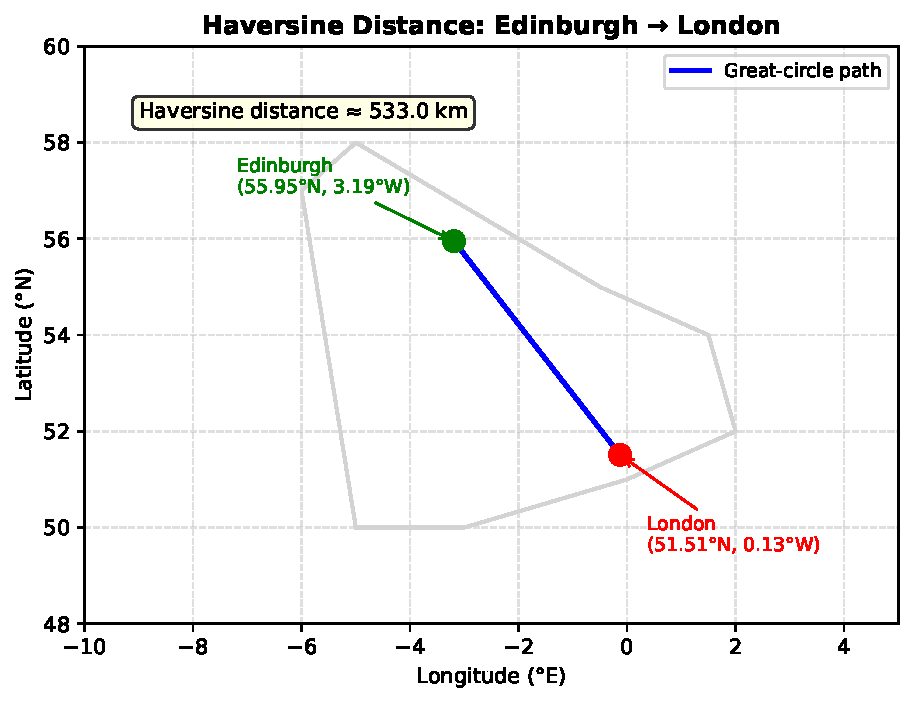
\includegraphics[width=0.72\textwidth]{haversine_example.pdf}
  \end{center}

  \framebreak

  \begin{center}
    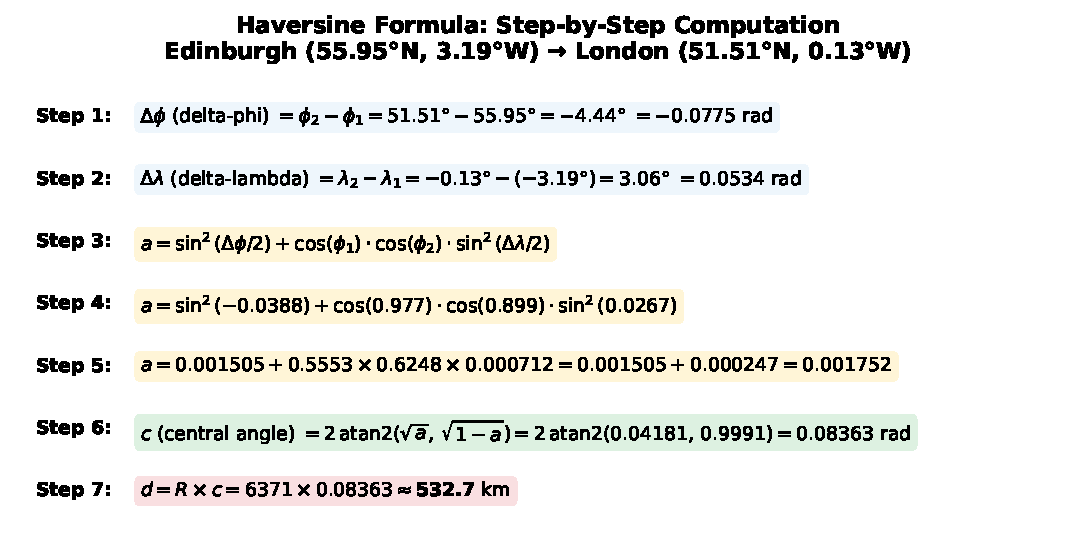
\includegraphics[width=0.88\textwidth]{haversine_steps.pdf}
  \end{center}

\end{frame}

% ────────────────────────────────────────────────────────────────
\begin{frame}[fragile]{Python: Computing Haversine Distance}
% ────────────────────────────────────────────────────────────────

\begin{lstlisting}[caption={Haversine distance function in Python}]
import math

def haversine(lat1: float, lon1: float,
              lat2: float, lon2: float) -> float:
    """
    Compute the great-circle distance between two points
    on the Earth's surface using the Haversine formula.

    Parameters
    ----------
    lat1, lon1 : float
        Latitude and longitude of point 1 in DEGREES.
    lat2, lon2 : float
        Latitude and longitude of point 2 in DEGREES.

    Returns
    -------
    float
        Great-circle distance in kilometres.
    """
    R = 6371.0  # Earth's mean radius in km

    # Convert degrees to radians
    phi1   = math.radians(lat1)
    phi2   = math.radians(lat2)
    dphi   = math.radians(lat2 - lat1)   # Delta-phi  (latitude difference)
    dlambda = math.radians(lon2 - lon1)  # Delta-lambda (longitude difference)

    # Haversine of the central angle
    a = (math.sin(dphi / 2) ** 2
         + math.cos(phi1) * math.cos(phi2) * math.sin(dlambda / 2) ** 2)

    # Central angle c (in radians)
    c = 2 * math.atan2(math.sqrt(a), math.sqrt(1 - a))

    return R * c   # Distance in km


# Example usage
dist = haversine(55.95, -3.19, 51.51, -0.13)
print(f"Edinburgh to London: {dist:.1f} km")
# Output: Edinburgh to London: 532.8 km
\end{lstlisting}

  This function accepts coordinates in \emph{degrees}, converts them to
  radians internally, and returns the distance in kilometres.
  The \texttt{math.atan2} function is used rather than \texttt{math.acos}
  to avoid numerical instability when the two points are nearly identical
  (i.e.\ when $a \approx 0$).

\end{frame}

% ================================================================
\section{7.4 Graph Theory and Networks}
% ================================================================

\begin{frame}[allowframebreaks]{7.4 Graph Theory: Foundations}

  Now that we know how to store geographic locations as coordinates,
  we need a data structure that represents the \emph{connectivity} of
  a road network.  A road network consists of junctions (where streets
  meet) connected by road segments (the streets themselves).  The
  mathematical object that captures exactly this structure --- a set
  of items with connections between them --- is called a \textbf{graph}.

  \begin{block}{Definition: Graph $G = (V, E)$}
    A graph $G$ is formally defined as an ordered pair $(V, E)$ where:
    \begin{itemize}
      \item $V$ (capital V) is the \textbf{set of vertices} (also called
            \emph{nodes}).  Each vertex represents an entity --- a road
            junction, a city, a person in a social network, etc.
      \item $E$ (capital E) is the \textbf{set of edges} (also called
            \emph{links} or \emph{arcs}).  Each edge represents a
            relationship or connection between two vertices.  An edge
            between vertices $v_i$ and $v_j$ (where $i$ and $j$ are
            indices identifying the vertices) is written as the pair
            $(v_i, v_j)$.
    \end{itemize}
  \end{block}

  \begin{center}
    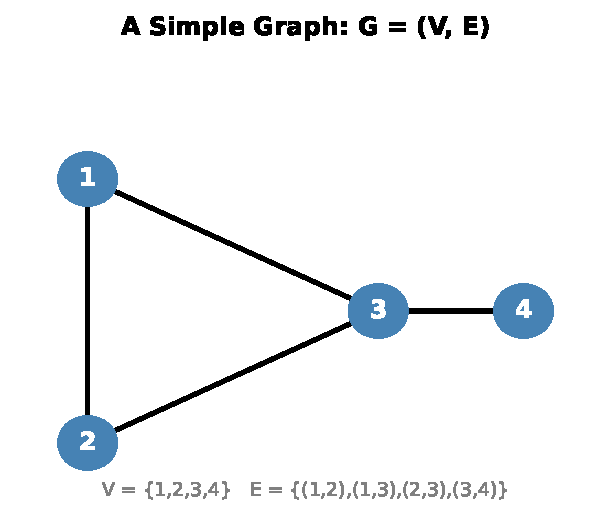
\includegraphics[width=0.45\textwidth]{simple_graph.pdf}
  \end{center}

  \framebreak

  \textbf{Reading the example graph.}
  In the figure above, we have four vertices $V = \{1, 2, 3, 4\}$
  and four edges $E = \{(1,2),\,(1,3),\,(2,3),\,(3,4)\}$.

  \begin{itemize}
    \item Vertex~1 has a connection to vertices~2 and~3, but \emph{not}
          to vertex~4.  This means, for example, that if junctions~1
          and~4 in a road network were represented by these vertices,
          you could not travel directly between them --- you would have
          to pass through vertex~3 first.
    \item Vertex~3 is the most ``central'' vertex here: it connects to
          all other vertices.  In the road-network analogy, this
          junction is the busiest, as all traffic must pass through it
          to get between the left cluster ($\{1, 2\}$) and vertex~4.
    \item Vertices~1 and~2 are connected to each other.  In graph
          terminology this means there is a \emph{direct} path between
          them.
  \end{itemize}

  \begin{alertblock}{Key Insight}
    A graph is an abstraction.  The same mathematical structure can
    represent road networks, social networks, computer networks,
    molecular structures, or any collection of entities with pairwise
    relationships.  The algorithms we develop for one domain (e.g.\
    finding shortest paths in a road network) transfer directly to
    other domains.
  \end{alertblock}

\end{frame}

% ────────────────────────────────────────────────────────────────
\begin{frame}[allowframebreaks]{7.4 Weighted Graphs}
% ────────────────────────────────────────────────────────────────

  In a plain (unweighted) graph, an edge simply records that two
  vertices are connected.  In a \textbf{weighted graph}, each edge
  also carries a numerical \textbf{weight} --- a number that
  quantifies the ``cost'' or ``strength'' of the connection.

  \begin{block}{Definition: Weighted Graph}
    A weighted graph $G = (V, E, W)$ extends the basic definition with
    \begin{itemize}
      \item $W$ (capital W): a \textbf{weight function} $W: E \to \mathbb{R}$
            that assigns a real number to each edge.  In road networks
            this weight is typically the \emph{distance} in metres or
            kilometres, or the \emph{travel time} in seconds.  In social
            networks it might be the \emph{level of interaction} between
            two users.
    \end{itemize}
  \end{block}

  \begin{center}
    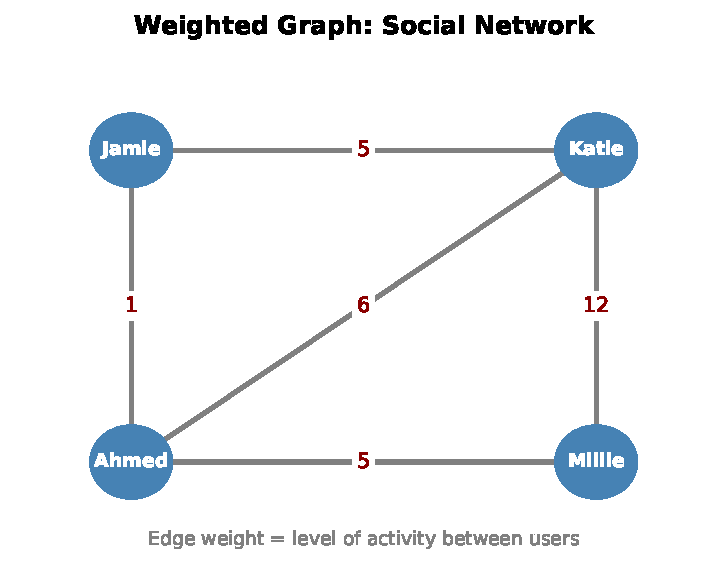
\includegraphics[width=0.52\textwidth]{weighted_social_graph.pdf}
  \end{center}

  \textbf{Reading the social-network example.}
  The four users Jamie, Katie, Ahmed, and Millie form a weighted graph
  in which the edge weight represents the frequency of interaction.
  Jamie and Katie have weight~5 (moderate activity).  Katie and
  Millie have weight~12 (the highest in the network --- they interact
  most frequently).  Jamie and Ahmed have weight~1 (rare interaction).
  Notice that \emph{Millie and Jamie are not connected by an edge at
  all}, meaning no recorded interaction between them.

  \framebreak

  \textbf{Weighted graphs for delivery optimisation.}
  In a road network weighted graph:
  \begin{itemize}
    \item Each \textbf{node} represents a road junction (intersection).
    \item Each \textbf{edge} represents a road segment connecting two junctions.
    \item The \textbf{weight} of an edge is typically the road distance
          (in metres) or the estimated travel time.
    \item Additional edge attributes might include the road name,
          classification (motorway, A-road, footpath), and speed limit.
    \item Node attributes might include whether the junction has traffic
          lights, or whether it is a roundabout.
  \end{itemize}

  When a routing algorithm (such as Dijkstra's algorithm) searches for
  the \emph{shortest path} between two locations, it traverses this
  weighted graph and finds the sequence of edges whose total weight
  (total distance or travel time) is minimised.

\end{frame}

% ────────────────────────────────────────────────────────────────
\begin{frame}[allowframebreaks]{7.4 Directed Graphs}
% ────────────────────────────────────────────────────────────────

  In an \textbf{undirected} graph, an edge $(v_i, v_j)$ implies that
  you can travel from $v_i$ to $v_j$ \emph{and} from $v_j$ to $v_i$
  --- the connection is symmetric.  Real road networks, however, have
  \textbf{one-way streets}: you may drive north along a street but
  \emph{not} south.  To model this, we use a \textbf{directed graph}
  (also called a \emph{digraph}).

  \begin{block}{Definition: Directed Graph}
    In a directed graph, each edge $(v_x, v_y)$ has a specific
    \textbf{direction}: it goes \emph{from} $v_x$ \emph{to} $v_y$,
    but \emph{not} necessarily the reverse.  The existence of edge
    $(v_x, v_y)$ does not imply the existence of edge $(v_y, v_x)$.
    When both directions exist, two separate directed edges are needed.
  \end{block}

  \begin{center}
    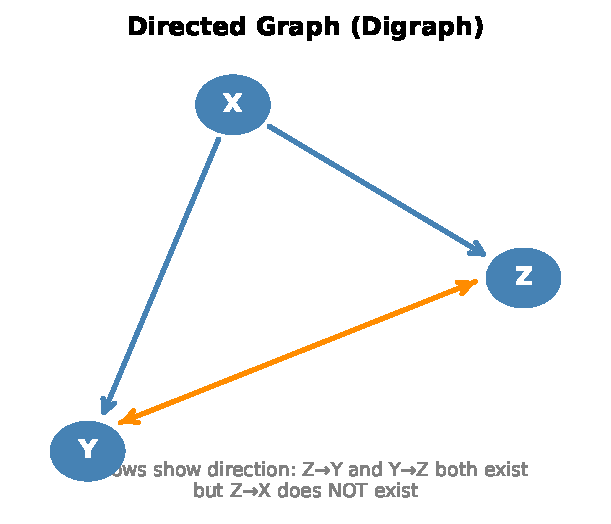
\includegraphics[width=0.42\textwidth]{directed_graph.pdf}
  \end{center}

  \framebreak

  \textbf{Reading the directed graph.}
  In the diagram, vertex~X connects to both Y and Z (arrows pointing
  outward from X).  Between Y and Z there are edges in \emph{both}
  directions (Y$\to$Z and Z$\to$Y), shown as two separate arrows.
  Crucially, there is \emph{no} edge from Z or Y back to X, and no
  edge from X directly to Y via Z.  A vehicle at Z cannot reach X in
  one hop.

  \textbf{Two edges for a two-way street.}
  For a bidirectional road segment between junctions $j_1$ and $j_2$,
  the graph model requires \emph{two} directed edges:
  $j_1 \to j_2$ and $j_2 \to j_1$.  Both can carry the same weight
  (road distance), but they could carry different weights if travel
  is faster in one direction (e.g.\ due to traffic light phasing).

  \begin{center}
    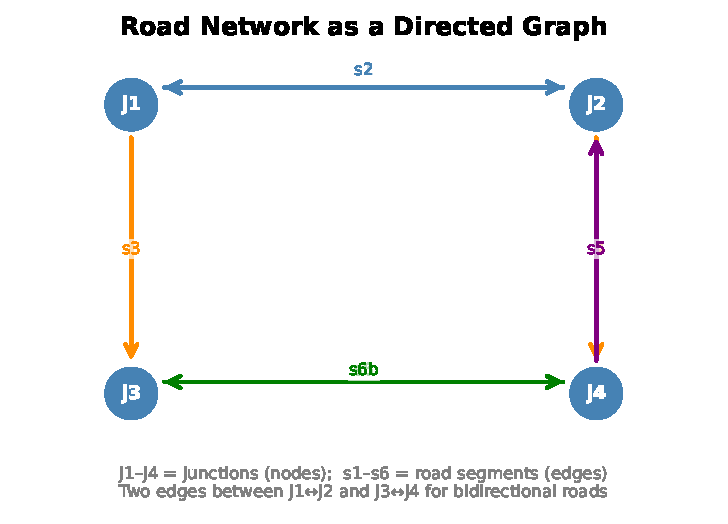
\includegraphics[width=0.60\textwidth]{road_network_graph.pdf}
  \end{center}

  {\footnotesize The road network graph with four junctions $j_1$--$j_4$ connected by
  directed road segments $s_1$--$s_6$.  Two directed edges between $j_1 \leftrightarrow j_2$
  model a two-way road; a single directed edge models a one-way street.}

  \framebreak

  \begin{block}{Edge Attributes in a Road Network Graph}
    When building a road network graph from vector data (e.g.\ OSM),
    the edges typically carry the following attributes:
    \begin{itemize}
      \item \textbf{Street name}: e.g.\ ``George Street''
      \item \textbf{Road number}: e.g.\ ``A1''
      \item \textbf{Road classification}: Motorway, Trunk, Primary,
            Secondary, Residential, Footpath, etc.
      \item \textbf{Speed limit}: in km/h or mph
      \item \textbf{Length}: in metres (computed from the GPS coordinates
            of the edge endpoints using the Haversine formula)
    \end{itemize}
    Junction \emph{nodes} may carry:
    \begin{itemize}
      \item \textbf{Traffic lights}: true/false
      \item \textbf{Roundabout}: true/false
    \end{itemize}
  \end{block}

  \begin{alertblock}{Key Insight}
    By storing a road network as a directed, weighted graph with
    rich edge attributes, we separate the \emph{data model}
    (the graph) from the \emph{algorithm} (the routing engine).
    This separation means we can swap in a different routing
    algorithm without changing the underlying data structure.
  \end{alertblock}

\end{frame}

% ────────────────────────────────────────────────────────────────
\begin{frame}[allowframebreaks]{7.4 Complex Junctions and Turn Restrictions}
% ────────────────────────────────────────────────────────────────

  Simple junctions can be modelled with a single node.  However,
  many real-world junctions have \textbf{restricted turns}: at a
  T-junction or crossroads, certain turn combinations may be
  prohibited --- for example, ``no right turn from Napier Street
  onto High Street''.  A single node cannot represent this, because
  the node model does not distinguish between entering the junction
  from different directions.

  \begin{block}{Modelling Complex Junctions with Multiple Nodes}
    A complex junction $j_1$ can be \emph{expanded} into a small
    sub-graph of internal nodes and edges, where:
    \begin{itemize}
      \item Each internal node represents a particular
            \emph{approach direction} into the junction
            (e.g.\ $j_{1a}$ = arriving via Napier Street,
            $j_{1b}$ = arriving via High Street eastbound,
            $j_{1c}$ = arriving via High Street westbound).
      \item Internal edges represent \emph{permitted} movements
            through the junction.
      \item A prohibited turn is simply absent --- there is no
            internal edge for that movement.
    \end{itemize}
  \end{block}

  \begin{center}
    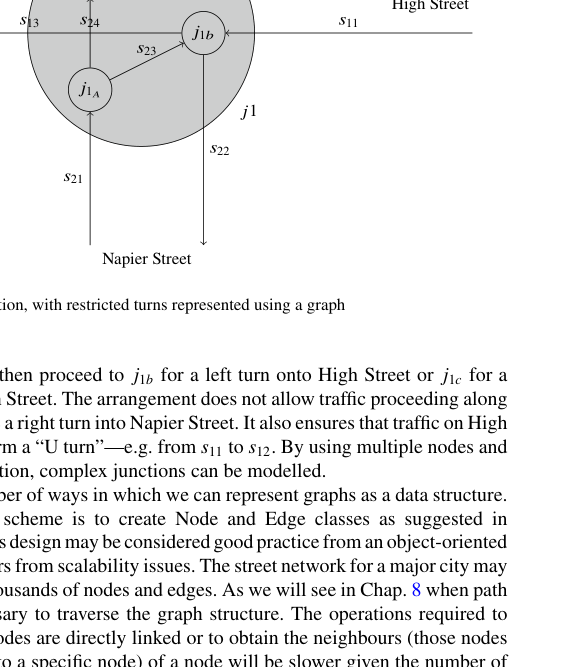
\includegraphics[width=0.58\textwidth]{fig_junction_turns_crop.png}
  \end{center}
  {\footnotesize Fig.~7.10 from the book: junction $j_1$ expanded into three internal
  nodes $j_{1a}$, $j_{1b}$, $j_{1c}$ connected by internal segments $s_{21}$--$s_{24}$,
  with external road segments $s_{11}$--$s_{14}$ connecting to the wider network.
  Traffic on High Street cannot turn right into Napier Street because no internal
  edge for that movement exists.}

  \framebreak

  \textbf{Example: reading the junction graph.}
  Vehicles arriving from Napier Street ($s_{21}$) enter at node $j_{1a}$.
  From $j_{1a}$ they may proceed to $j_{1b}$ (for a left turn onto
  High Street heading east) or $j_{1c}$ (for a right turn onto
  High Street heading west).
  However, traffic already travelling \emph{along} High Street
  (entering at $j_{1b}$ or $j_{1c}$) cannot turn right into Napier
  Street, because the arc from $j_{1b}$ or $j_{1c}$ to $j_{1a}$ is
  simply not present in the graph.
  The junction model also prevents U-turns by not including edges from
  $j_{1b}$ back to $j_{1c}$ or vice versa.

  \begin{alertblock}{Key Insight}
    This multi-node junction model demonstrates the power and
    flexibility of graph representations.  A constraint as complex
    as a restricted turn at a specific junction is encoded simply
    as the \emph{absence of an edge} --- no special-purpose data
    structure or algorithm modification is required.
  \end{alertblock}

\end{frame}

% ────────────────────────────────────────────────────────────────
\begin{frame}[allowframebreaks]{7.4 Graph Data Structures}
% ────────────────────────────────────────────────────────────────

  We now know \emph{conceptually} what a graph is.  The question is
  how to represent it efficiently in computer memory.  There are two
  principal choices: the \textbf{object-oriented representation} and
  the \textbf{adjacency matrix}.

  \begin{block}{Option 1: Object-Oriented (Node and Edge Classes)}
    The most natural approach from an object-oriented programming
    perspective is to define classes \texttt{Node}, \texttt{Edge},
    and \texttt{Graph}:
    \begin{itemize}
      \item A \texttt{Node} object stores its identifier, coordinates,
            and a list of incident edges.
      \item An \texttt{Edge} object stores its weight, its source
            \texttt{Node}, and its destination \texttt{Node}.
      \item A \texttt{Graph} object holds a list of all nodes and a
            list of all edges.
    \end{itemize}
    This design is clean and intuitive.  However, for a major city's
    road network (potentially tens of thousands of nodes and edges),
    the overhead of managing tens of thousands of individual Python
    objects --- and navigating between them via object references ---
    can make operations slow.
  \end{block}

  \framebreak

  \begin{block}{Option 2: Adjacency Matrix}
    An alternative representation uses a 2D matrix (a 2D array or
    list-of-lists in Python) of size $n \times n$, where $n$ is the
    number of nodes in the graph.

    \begin{itemize}
      \item The cell at row $i$, column $j$ of the matrix stores $1$
            (or the edge weight) if there is an edge from node $v_i$
            to node $v_j$.
      \item If there is no direct connection between $v_i$ and $v_j$,
            the cell stores $0$ (or $-1$ to signal ``no direct link'').
    \end{itemize}

    \textbf{Advantages:}
    \begin{itemize}
      \item Checking whether two nodes are connected is an $O(1)$
            operation (a single array lookup).
      \item Finding all neighbours of a node is an $O(n)$ scan
            of one row.
      \item Numerically efficient --- a large array is far cheaper
            in memory and access time than a large collection of
            Python objects.
    \end{itemize}

    \textbf{Disadvantage:} For a graph with $n$ nodes, the matrix
    uses $n^2$ cells.  A network with 10{,}000 nodes requires a
    $100{,}000{,}000$-cell matrix, which consumes a great deal of
    memory even if most roads do not directly connect to each other
    (i.e.\ the matrix is \emph{sparse}).
  \end{block}

  \framebreak

  \begin{exampleblock}{Worked Example: Adjacency Matrix for $j_1$--$j_4$}
    Consider the directed road network with junctions $j_1, j_2, j_3, j_4$
    (Fig.~7.9 from the book).  The directed edges are:
    $j_1 \to j_2$,\; $j_2 \to j_1$ (bidirectional top road),\;
    $j_1 \to j_3$ (one-way left road),\;
    $j_2 \to j_4$ (one-way right road),\;
    $j_4 \to j_2$ (one-way returning),\;
    $j_3 \leftrightarrow j_4$ (bidirectional bottom road).

    \vspace{0.4em}
    \renewcommand{\arraystretch}{1.3}
    \begin{tabular}{c|cccc}
      & \textbf{j1} & \textbf{j2} & \textbf{j3} & \textbf{j4} \\
      \hline
      \textbf{j1} & 0 & 1 & 1 & 0 \\
      \textbf{j2} & 1 & 0 & 0 & 1 \\
      \textbf{j3} & 0 & 0 & 0 & 1 \\
      \textbf{j4} & 0 & 1 & 1 & 0 \\
    \end{tabular}
    \vspace{0.4em}

    Row $i$ tells you where node $j_i$ can \emph{go to}.
    Column $j$ tells you which nodes can \emph{reach} $j_j$.
    For example, row~j3 has only one ``1'' (in column j4), confirming
    that the only direct exit from junction $j_3$ is to $j_4$.
    Cell (j1, j4) is~0, confirming no direct road from $j_1$ to $j_4$.
  \end{exampleblock}

  \begin{center}
    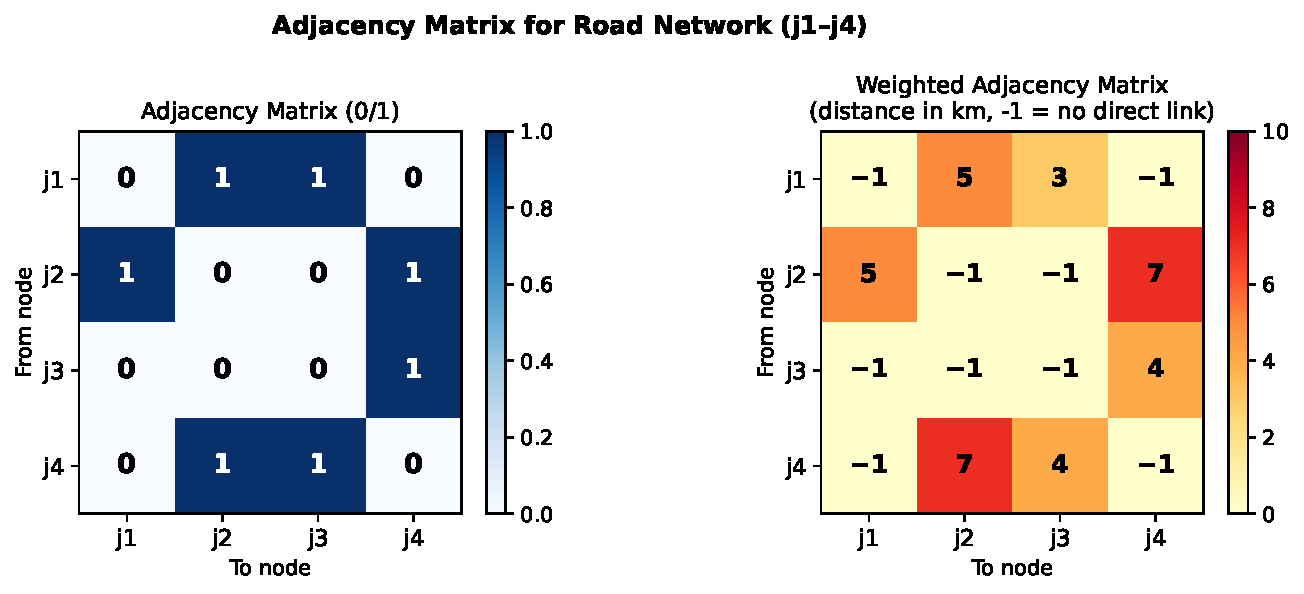
\includegraphics[width=0.80\textwidth]{adjacency_matrix.pdf}
  \end{center}

  \framebreak

  \textbf{Weighted adjacency matrix.}
  A useful modification is to replace the binary 0/1 entries with
  actual edge weights.  For roads this would be the distance in
  metres.  Cells where no direct connection exists are set to $-1$
  (to distinguish ``no connection'' from a zero-length edge).

  \begin{block}{Using the Weighted Adjacency Matrix}
    \begin{itemize}
      \item \textbf{Checking connectivity}: cell $(i, j) > 0$ means
            there is a direct road from junction $i$ to $j$.
      \item \textbf{Getting the distance}: cell $(i, j)$ gives the
            road length directly.
      \item \textbf{Finding neighbours}: scan row $i$ and collect
            all column indices $j$ where the cell is $> 0$.
      \item In many routing algorithms (e.g.\ Dijkstra's), the
            adjacency matrix is the primary lookup table: at each step,
            the algorithm reads $A[i][j]$ to get the cost of moving
            from junction $i$ to $j$.
    \end{itemize}
  \end{block}

  \begin{center}
    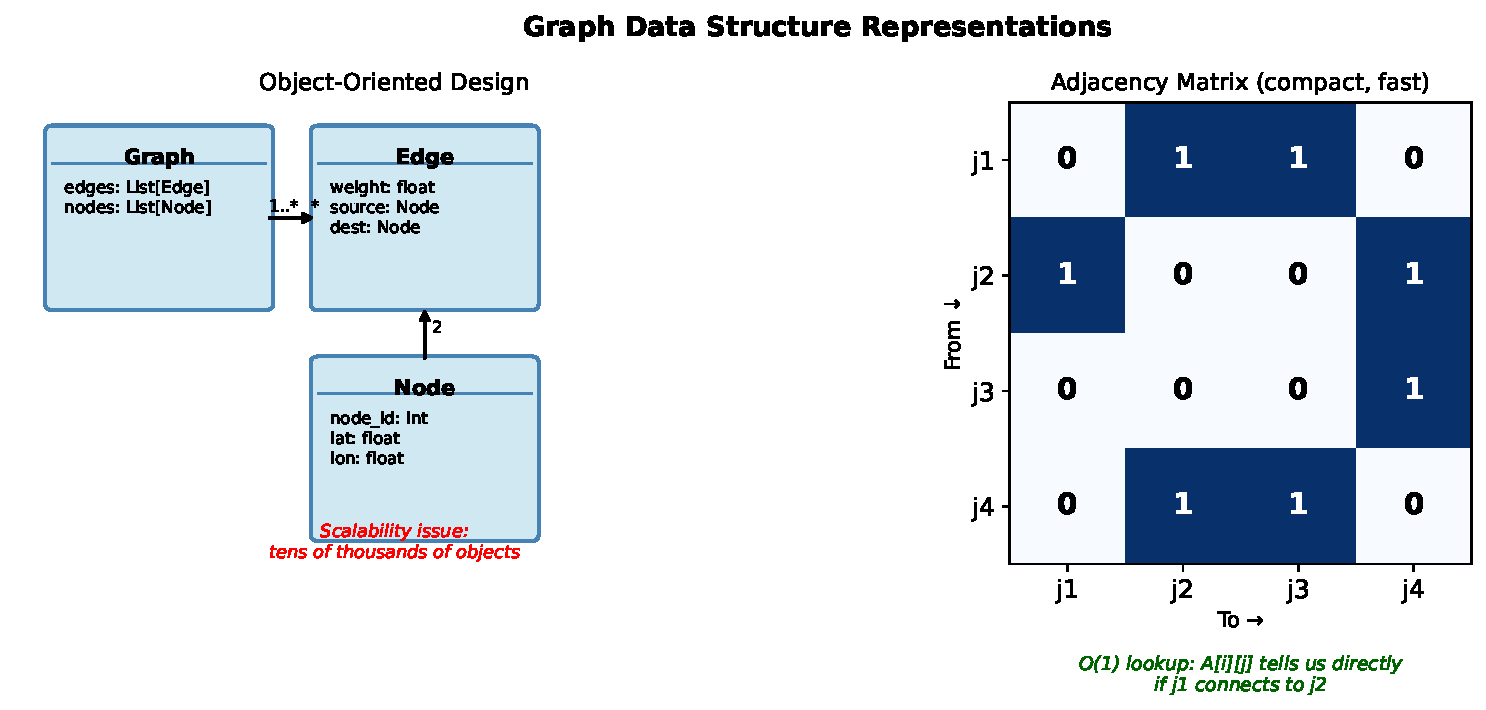
\includegraphics[width=0.80\textwidth]{graph_representations.pdf}
  \end{center}

\end{frame}

% ────────────────────────────────────────────────────────────────
\begin{frame}[fragile]{Python: Building a Graph with an Adjacency Matrix}
% ────────────────────────────────────────────────────────────────

\begin{lstlisting}[caption={Graph class using an adjacency matrix}]
import numpy as np

class Graph:
    """
    A directed, weighted graph represented by an adjacency matrix.
    Nodes are labelled 0 to n-1 internally.
    """
    def __init__(self, n: int):
        self.n = n
        # -1 means no direct connection; 0 or positive means there is one
        self.adj = -1 * np.ones((n, n), dtype=float)
        np.fill_diagonal(self.adj, 0)   # Distance from a node to itself = 0

    def add_edge(self, src: int, dst: int, weight: float):
        """Add a directed edge from src to dst with the given weight."""
        self.adj[src][dst] = weight

    def get_weight(self, src: int, dst: int) -> float:
        """Return edge weight, or -1 if no direct connection."""
        return self.adj[src][dst]

    def neighbours(self, node: int) -> list:
        """Return list of (neighbour_index, edge_weight) pairs."""
        return [(j, self.adj[node][j])
                for j in range(self.n)
                if self.adj[node][j] >= 0 and j != node]

# Build the j1-j4 road network (nodes indexed 0=j1, 1=j2, 2=j3, 3=j4)
g = Graph(4)
g.add_edge(0, 1, 5.0)   # j1 -> j2, 5 km
g.add_edge(1, 0, 5.0)   # j2 -> j1  (bidirectional)
g.add_edge(0, 2, 3.0)   # j1 -> j3, 3 km (one-way)
g.add_edge(1, 3, 7.0)   # j2 -> j4, 7 km
g.add_edge(3, 1, 7.0)   # j4 -> j2  (bidirectional)
g.add_edge(2, 3, 4.0)   # j3 -> j4, 4 km
g.add_edge(3, 2, 4.0)   # j4 -> j3  (bidirectional)

print("Adjacency matrix:")
print(g.adj)
print()
print("Neighbours of j1 (node 0):", g.neighbours(0))
# Output: Neighbours of j1 (node 0): [(1, 5.0), (2, 3.0)]
\end{lstlisting}

\end{frame}

% ────────────────────────────────────────────────────────────────
\begin{frame}[fragile]{Python: Building a Road Network with OSMnx}
% ────────────────────────────────────────────────────────────────

  In practice, we rarely build graph objects by hand.  The
  \texttt{osmnx} library downloads road network data from
  OpenStreetMap and constructs a \texttt{networkx} directed graph
  automatically.  Each node corresponds to a road junction
  and carries latitude/longitude attributes; each edge corresponds
  to a road segment and carries distance, speed limit, and other
  metadata.

\begin{lstlisting}[caption={Building and querying an OSM road network graph}]
import osmnx as ox
import networkx as nx

# Download the driveable road network for central Edinburgh
G = ox.graph_from_place("Edinburgh City Centre, UK",
                         network_type="drive")

# G is a networkx MultiDiGraph (directed, multi-edge)
print(f"Nodes: {G.number_of_nodes()}")
print(f"Edges: {G.number_of_edges()}")

# Get node attributes (latitude and longitude)
node_id = list(G.nodes)[0]
attrs = G.nodes[node_id]
print(f"Node {node_id}: lat={attrs['y']:.5f}, lon={attrs['x']:.5f}")

# Get edge attributes
u, v, key, data = list(G.edges(keys=True, data=True))[0]
print(f"Edge {u}->{v}: length={data.get('length', '?')} m, "
      f"name={data.get('name', 'unnamed')}, "
      f"maxspeed={data.get('maxspeed', 'n/a')}")

# Find shortest path by distance between two nodes
orig = list(G.nodes)[0]
dest = list(G.nodes)[-1]
path = nx.shortest_path(G, orig, dest, weight='length')
total_dist = sum(G[path[i]][path[i+1]][0].get('length', 0)
                 for i in range(len(path)-1))
print(f"Shortest path has {len(path)} nodes, "
      f"total distance {total_dist/1000:.2f} km")
\end{lstlisting}

\end{frame}

% ────────────────────────────────────────────────────────────────
\begin{frame}[allowframebreaks]{7.4 Road Network as a Graph: Edinburgh Example}
% ────────────────────────────────────────────────────────────────

  The following figure shows a satellite image of part of Edinburgh
  alongside the graph representation generated from OpenStreetMap data
  for the same area.  Each blue dot is a node (road junction); each
  line is an edge (road segment).

  \begin{center}
    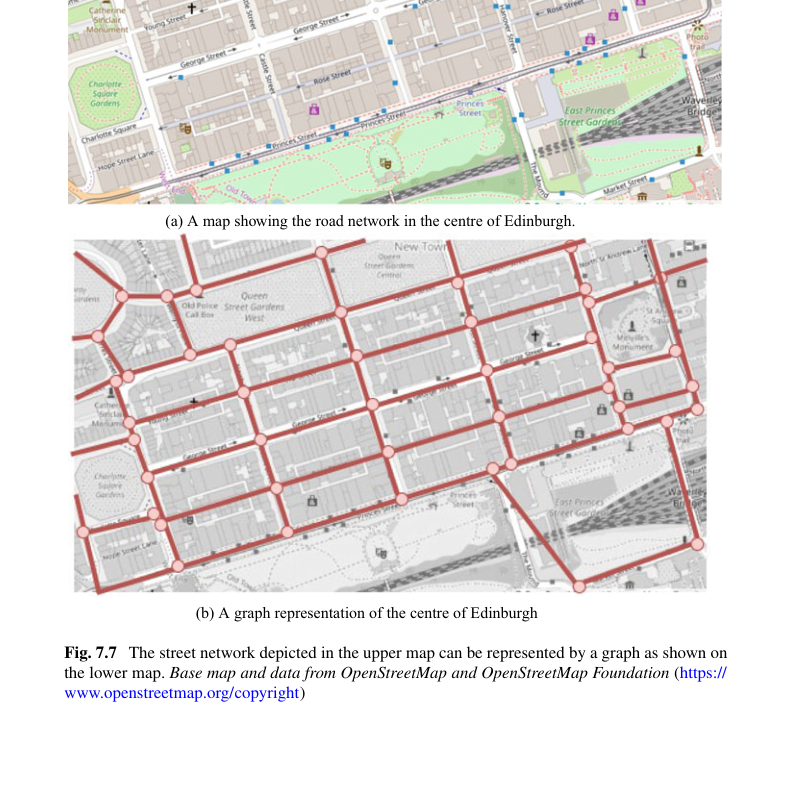
\includegraphics[width=0.90\textwidth]{fig_edinburgh_map_crop.png}
  \end{center}

  \vspace{0.3em}
  Comparing the two images illustrates several important points:
  \begin{itemize}
    \item Major intersections appear as nodes with high
          \emph{degree} (many edges connecting to them).
    \item Small side streets and alleyways create many low-degree
          nodes (perhaps only two edges: entry and exit).
    \item The graph captures the topological structure (connectivity)
          of the network but not the exact spatial geometry of curved
          roads --- each edge is a straight line between the endpoint
          coordinates, even if the actual road curves.
    \item In OSM, roads with many bends are represented as
          \emph{ways} consisting of multiple sequential coordinate
          pairs (``way nodes''), each of which becomes a node in the
          graph.  This allows the graph to approximate road geometry
          as a polyline.
  \end{itemize}

  \begin{alertblock}{Key Insight}
    The power of the graph representation is that it makes
    large-scale route optimisation tractable.  A delivery
    optimisation algorithm does not need to reason about satellite
    imagery or pixel colours --- it only needs to traverse the
    graph, summing edge weights along candidate routes.
  \end{alertblock}

\end{frame}

% ================================================================
\section{7.5 Conclusions}
% ================================================================

\begin{frame}[allowframebreaks]{7.5 Conclusions}

  This chapter has described the data types and structures that are
  commonly used in geographical information systems.  These form a
  necessary part of our problem models when we come to optimise
  delivery routes.

  \begin{block}{Summary of Key Concepts}
    \begin{enumerate}
      \item \textbf{History of mapping}: The desire to create accurate
            maps is ancient, but the digital revolution has made
            planetary-scale, on-demand geospatial data available to
            everyone.  OpenStreetMap is a freely available, volunteer-built
            global map used widely in delivery and logistics applications.

      \item \textbf{Raster vs.\ vector}: Map data may be stored as raster
            pixel images or as vector geometric data.  A rendering
            algorithm converts vector data into the raster images that
            screens display.  Vector data is preferred for GIS
            applications because it is compact, scalable, and can carry
            rich metadata.

      \item \textbf{Coordinate systems}: The latitude/longitude system
            (WGS84) provides a global framework for specifying locations.
            The Haversine formula gives the great-circle (straight-line
            surface) distance between any two coordinate points on the
            Earth.

      \item \textbf{Graph theory}: A directed, weighted graph $G = (V, E)$
            is the natural data structure for representing a road network.
            Junctions become nodes, road segments become directed edges,
            and distances or travel times become edge weights.  The
            adjacency matrix provides a computationally efficient
            implementation.
    \end{enumerate}
  \end{block}

  \framebreak

  \begin{alertblock}{Looking Ahead}
    With the road network stored as a graph, we are ready to apply
    \textbf{routing algorithms} --- methods for finding efficient
    paths through the graph.  Chapter~8 will introduce the most
    important such algorithms, including Dijkstra's shortest-path
    algorithm, and explain how they are used within delivery
    optimisation frameworks.
  \end{alertblock}

  \begin{block}{Practical Python Ecosystem for GeoSpatial Work}
    The following Python libraries together provide a complete pipeline
    from raw geospatial data to an optimisable graph:
    \begin{itemize}
      \item \textbf{osmnx}: downloads road networks from OpenStreetMap
            and returns \texttt{networkx} graph objects.
      \item \textbf{networkx}: general-purpose graph library;
            includes Dijkstra's algorithm, betweenness centrality,
            and many other graph algorithms.
      \item \textbf{shapely}: geometric operations on vector shapes
            (intersection, union, buffering).
      \item \textbf{geopandas}: extends pandas DataFrames with a
            geometry column; supports reading/writing all major
            vector formats (GeoJSON, Shapefile, etc.).
      \item \textbf{folium} / \textbf{leaflet.js}: interactive map
            visualisation in a browser.
      \item \textbf{matplotlib}: static map plots, graph diagrams.
    \end{itemize}
  \end{block}

\end{frame}

% ────────────────────────────────────────────────────────────────
\begin{frame}[fragile]{Python: End-to-End Pipeline Summary}
% ────────────────────────────────────────────────────────────────

\begin{lstlisting}[caption={Complete pipeline: OSM data to shortest-path result}]
import osmnx as ox
import networkx as nx
import math

def haversine(lat1, lon1, lat2, lon2):
    R = 6371.0
    phi1, phi2 = math.radians(lat1), math.radians(lat2)
    dphi = math.radians(lat2 - lat1)
    dlam = math.radians(lon2 - lon1)
    a = math.sin(dphi/2)**2 + math.cos(phi1)*math.cos(phi2)*math.sin(dlam/2)**2
    return R * 2 * math.atan2(math.sqrt(a), math.sqrt(1 - a))

# Step 1: Download road network from OSM
G = ox.graph_from_place("Edinburgh, UK", network_type="drive")
print(f"Network: {G.number_of_nodes()} nodes, {G.number_of_edges()} edges")

# Step 2: Find the nearest graph nodes to two address coordinates
# (lat, lon) of two delivery locations
delivery_A = (55.9533, -3.1883)   # Edinburgh city centre
delivery_B = (55.9441, -3.2024)   # Tollcross area

node_A = ox.nearest_nodes(G, X=delivery_A[1], Y=delivery_A[0])
node_B = ox.nearest_nodes(G, X=delivery_B[1], Y=delivery_B[0])

# Step 3: Compute shortest path by road distance
route = nx.shortest_path(G, node_A, node_B, weight='length')
route_length = sum(G[route[i]][route[i+1]][0]['length']
                   for i in range(len(route)-1))

# Step 4: Compare to straight-line (Haversine) distance
crow_flies = haversine(*delivery_A, *delivery_B) * 1000  # convert km -> m

print(f"Shortest road path: {route_length:.0f} m ({len(route)} junctions)")
print(f"Straight-line dist: {crow_flies:.0f} m")
print(f"Detour factor     : {route_length/crow_flies:.2f}x")
# Typical output for urban areas: Detour factor 1.3x - 1.6x
\end{lstlisting}

  The ``detour factor'' (road distance divided by straight-line
  distance) is typically 1.2--1.5 for urban road networks.  This is
  an important parameter in delivery optimisation: a model that uses
  only straight-line distances will systematically underestimate
  route lengths by 20--50\%.

\end{frame}

% ────────────────────────────────────────────────────────────────
\begin{frame}{Chapter 7 Summary Card}
% ────────────────────────────────────────────────────────────────
  \begin{columns}[t]
    \begin{column}{0.48\textwidth}
      \begin{block}{Concepts}
        \begin{itemize}
          \item Raster: pixel grid, resolution-limited
          \item Vector: geometry + metadata, scalable
          \item WGS84: global lat/lon coordinate standard
          \item Haversine: great-circle distance formula
          \item Graph $G=(V,E)$: nodes + edges
          \item Weighted graph: edges carry distances/times
          \item Directed graph: models one-way streets
          \item Adjacency matrix: $O(1)$ connectivity lookup
        \end{itemize}
      \end{block}
    \end{column}
    \begin{column}{0.48\textwidth}
      \begin{block}{Key Formulas}
        \textbf{Haversine:}
        \[
          a = \sin^2\!\tfrac{\Delta\phi}{2} +
              \cos\phi_1 \cos\phi_2 \sin^2\!\tfrac{\Delta\lambda}{2}
        \]
        \[
          d = 2R\,\mathrm{atan2}\!\left(\sqrt{a},\sqrt{1-a}\right)
        \]
        \textbf{Graph definition:}
        \[
          G = (V,\, E)
        \]
        $V$ = vertices (junctions), $E$ = edges (roads)
      \end{block}
      \begin{block}{Python Libraries}
        \texttt{osmnx}, \texttt{networkx}, \texttt{geopandas},
        \texttt{shapely}, \texttt{folium}
      \end{block}
    \end{column}
  \end{columns}
\end{frame}

% ================================================================
\end{document}
% ================================================================
